% !TEX root = % !TEX root = /Users/nai1ka/Projects/PerfX/Thesis/thesis.tex
\chapter{Implementation}
\label{chap:impl}

This chapter describes how the design from Chapter~\ref{chap:met} was turned into working software.\footnote{The source code is available at \url{https://github.com/nai1ka/PerfX}.} Section~\ref{sec:sdk_impl} covers the mobile SDK, from initialization to the individual collectors and the buffering and transmission pipeline. Section~\ref{sec:backend_impl} describes the Backend, focusing on user management and the ingestion path. Section~\ref{sec:regression_impl} explains the regression detection pipeline in detail. Section~\ref{sec:frontend_impl} then walks through the frontend web application and its main features.

\section{Mobile SDK Implementation}
\label{sec:sdk_impl}

The mobile part of the monitoring system was implemented as an Android library written in Kotlin. Kotlin was chosen because it is the official, recommended language for Android development~\cite{KotlinFirst}.


The SDK is distributed through a Maven repository, which allows developers to add it to their project easily by adding s dependency to their \texttt{build.gradle} file.

\subsection{Initialization and Lifecycle Management}

One of the requirements for the SDK was to make the integration as simple as possible for developers. To achieve this, the entire setup is done with a single call to the \texttt{PerfX.initialize()} method inside the application class. The developer only needs to provide the application context and a unique project ID.

Initialization runs a short sequence of steps. The \texttt{AppInfoProvider} collects device and app metadata (OS version, device model, app version). The SDK then opens the local Room database (\texttt{MetricDatabase}), starts the background sync manager, and creates the metric collectors. Finally, the SDK registers an \texttt{Application.ActivityLifecycleCallbacks} listener so it can follow the active screen and pause network sync while the app sits in the background, which saves battery.

\begin{lstlisting}[language=Kotlin, caption={SDK Initialization}]
fun initialize(application: Application, projectId: String) {
    if (isRunning) return

    appInfo = AppInfoProvider().get(application, projectId)
    db = MetricDatabase.getInstance(application)
    SyncManager.startPeriodicSync(application)

    // ... Collector initialization (described below)

    registerActivityCallback(application)
    isRunning = true
}
\end{lstlisting}

\subsection{Performance Metrics Collectors}

Each metric collector extends a common abstract class called \texttt{PerformanceCollector}. This class defines a single \texttt{collect()} method that returns a Kotlin \texttt{Flow} of \texttt{Metric} objects, which allows the SDK to treat all collectors in a uniform way.

\begin{lstlisting}[language=Kotlin, caption={PerformanceCollector Abstract Class}]
internal abstract class PerformanceCollector {
    abstract fun collect(intervalMs: Long): Flow<Metric>
    abstract fun stop()
}
\end{lstlisting}

All individual metric streams are merged into a single \texttt{Flow} inside the \texttt{MetricsRepository} class. This design makes it easy to add new collectors in the future without changing the rest of the pipeline.

\textbf{1. Memory Collector}

The \texttt{RamCollector} runs on a background thread and measures the memory footprint of the application at a fixed sampling interval. It uses two Android APIs: \texttt{Debug.getMemoryInfo()} to get the total PSS (Proportional Set Size) of the process, and the Java \texttt{Runtime} to calculate the current Java heap usage. The Java heap usage is calculated as the difference between the total allocated heap and the currently free heap. This value is what gets emitted as the metric, because it reflects the memory actually used by the application code.

\begin{lstlisting}[language=Kotlin, caption={Memory Collector Implementation}]
val memoryInfo = Debug.MemoryInfo()
Debug.getMemoryInfo(memoryInfo)

val runtime = Runtime.getRuntime()
val javaHeapUsedMb = (runtime.totalMemory() - runtime.freeMemory()) / (1024.0 * 1024.0)
val pssMb = memoryInfo.totalPss / 1024.0

emit(Metric.MemoryUsage(timestamp = System.currentTimeMillis(), value = javaHeapUsedMb))
\end{lstlisting}

\textbf{2. CPU Collector}

Because modern Android versions restrict direct access to the \texttt{/proc/stat} file for security reasons, the \texttt{CpuCollector} uses the \texttt{android.os.Process} API instead. From this API it reads the accumulated CPU time of the application process at two points, one sampling interval apart. The CPU percentage is the CPU time used during that interval divided by the wall-clock length of the interval:

\begin{equation}
    CPU\% = \frac{\Delta CPU_{process}}{\Delta t_{wall}} \cdot 100
\end{equation}

This ratio expresses how much CPU time the application used relative to real time, so the values stay comparable across devices with different core counts.

\textbf{3. Frame Time Collector}

Frame rendering time is captured through a \texttt{Choreographer.FrameCallback} registered on the main thread. Android invokes this callback just before each new frame is drawn and passes the frame timestamp in nanoseconds. Subtracting the timestamps of two consecutive callbacks gives the raw frame time. Individual frame times are accumulated over a fixed interval and then averaged before being emitted as a single metric. This aggregation reduces the number of data points that need to be stored and transmitted, while still capturing the overall rendering performance of the window.

\begin{lstlisting}[language=Kotlin, caption={Frame Time Collector: core measurement}]
val callback = Choreographer.FrameCallback { frameTimeNs ->
    if (lastFrameTimeNs != 0L) {
        val deltaMs = (frameTimeNs - lastFrameTimeNs) / 1_000_000.0
        if (deltaMs >= 0.0) {
            frameCount++
            totalFrameTimeMs += deltaMs
        }
    }
    lastFrameTimeNs = frameTimeNs
    Choreographer.getInstance().postFrameCallback(frameCallback)
}

// Emitted every intervalMs
val avgFrameTime = if (frameCount > 0) totalFrameTimeMs / frameCount else 0.0
emit(Metric.FrameTime(timestamp = System.currentTimeMillis(), value = avgFrameTime))
\end{lstlisting}

\textbf{4. Startup Time Collector}

Startup time is measured by recording the timestamp at the moment the application process starts and comparing it to the timestamp of the first fully drawn frame. The SDK uses the \texttt{reportFullyDrawn()} API to detect when the first screen has finished rendering. The difference between these two timestamps is reported as the startup time.

\textbf{5. Interaction Delay Collector}

User interaction delay is measured by intercepting touch events on the root view of each activity. When a touch event is received, its timestamp is recorded. The delay is then calculated as the time between the touch event and the first frame rendered after the event was processed, which is detected using the \texttt{Choreographer} callback.

\textbf{6. ANR Detector}

The SDK detects ANR events using a watchdog pattern. A background thread posts a short task to the main thread's \texttt{Handler} and waits for it. If the task does not run within the timeout (5 seconds by default, matching the official Android documentation~\cite{AndroidANR}), the watchdog treats the main thread as blocked and records an ANR. The approach needs no special permissions and works on every Android version.

\begin{lstlisting}[language=Kotlin, caption={ANR Watchdog: detection logic}]
val mainHandler = Handler(Looper.getMainLooper())
var mainThreadResponded = false

mainHandler.post { mainThreadResponded = true }
Thread.sleep(ANR_TIMEOUT_MS)

if (!mainThreadResponded) {
    emit(Metric.Anr(timestamp = System.currentTimeMillis()))
}
\end{lstlisting}

\subsection{Data Buffering and Network Transmission}

The SDK uses a two-tier buffering approach to make sure that no metrics are lost if the application crashes or the network is temporarily unavailable.

\textbf{Tier 1: In-Memory Buffer}

As metrics arrive from the various collectors, they are first stored in a \texttt{ConcurrentLinkedQueue}. This structure was chosen because several collectors write at the same time from different background threads, and a plain list could lead to race conditions. A \texttt{ConcurrentLinkedQueue} handles concurrent access safely without explicit locks, which keeps the overhead low.

When the number of items in the memory buffer reaches a predefined limit (\texttt{MEMORY\_LIMIT}), the buffer is flushed to disk.

\begin{lstlisting}[language=Kotlin, caption={In-Memory Buffering}]
flow.collect { metric ->
    memoryBuffer.add(metric)
    memoryBufferSize += 1

    if (memoryBufferSize >= Constants.MEMORY_LIMIT) {
        flushToDisk(db, context)
        memoryBufferSize = 0
    }
}
\end{lstlisting}

\textbf{Tier 2: Disk Storage and Network Synchronization}

On a flush, the metrics move to a local SQLite database managed by the Room library. Each record is stored together with the name of the screen that was visible at the time, which the lifecycle callback registered during initialization keeps track of.

Once the database holds \texttt{DISK\_LIMIT} records, the SDK starts a network synchronization immediately. A background job also runs every 15 minutes and uploads whatever is left, even if that limit has not been reached, so metrics are still sent when the application is used only rarely.

The network layer uses Retrofit and OkHttp. The SDK reads a batch of records from the database, serializes it to JSON with Kotlinx Serialization, and sends it to the backend in a single HTTP POST request. On success, the uploaded records are deleted from the local database. On failure, they stay on disk and are retried at the next synchronization.

\begin{lstlisting}[language=Kotlin, caption={Network Synchronization}]
val batchApi = BatchApi(
    appInfo = PerfX.appInfo,
    metrics = batch.map { it.mapToApi() }
)

val response = NetworkClient.api.uploadBatch(batchApi)

if (response.isSuccessful) {
    db.metricDao().deleteMetrics(batch.map { it.id })
}
\end{lstlisting}

\section{Backend Implementation}
\label{sec:backend_impl}

The backend was built in Kotlin with the Ktor framework. Ktor is lightweight and asynchronous, which fits a REST API well. It serves each request on a coroutine, so it can handle many connections at once without blocking threads.

It relies on two databases: PostgreSQL for relational data such as user accounts and project metadata, and ClickHouse for the time-series performance metrics.

\subsection{User and Project Management}

PostgreSQL holds the user accounts, projects, version releases, and detected regressions, following the relational data model shown in Chapter~\ref{chap:met} (Figure~\ref{fig:postgres_schema}).

Passwords are hashed with BCrypt before they are stored. At login, the server checks the supplied password against the stored hash, and on success it issues a JSON Web Token (JWT). Every later request to the API must carry this token, which keeps each user's data accessible only to that user.


To create a project, a developer submits a name and an Android package name, and the server rejects either one if it is already taken. Once the project passes this check, it is saved and linked to the developer's account. A background job periodically refreshes the \texttt{version\_releases} catalogue from ClickHouse, recording each observed version code together with its first-seen time and accumulated sample count. The dashboard uses this catalogue to list the releases of a project.

\subsection{Data Ingestion}
\label{sec:ingestion}

The data ingestion endpoint is the most performance-critical part of the backend, because the mobile SDKs from many users can send large numbers of metrics at the same time. Storing this data in PostgreSQL would not be efficient enough for this workload. For this reason, all performance metrics are stored in ClickHouse, which is a column-oriented database optimized for fast batch insertions and analytical range queries over time~\cite{schulze2024clickhouse}.

The \texttt{metric\_records} table was designed to support the queries needed by the regression detection pipeline efficiently. The table uses the \texttt{MergeTree} engine, which is optimized for fast insertions and range scans. The data is partitioned by date so that queries over a recent time window only scan the relevant partitions. The primary sort key is \texttt{(project\_id, metric\_id, ts)}, which makes range queries over time for a specific project and metric very fast.

\newpage

\begin{lstlisting}[language=SQL, caption={ClickHouse metric\_records table schema}]
CREATE TABLE IF NOT EXISTS metrics.metric_records
(
    project_id    String,
    package_name  String,
    ts            DateTime64(3, 'UTC'),
    metric_id     LowCardinality(String),
    screen_name   LowCardinality(String),
    value         Float64,
    app_version   LowCardinality(String),
    os_version    LowCardinality(String),
    device_model  LowCardinality(String),
    device_cohort LowCardinality(String) DEFAULT 'Unknown',
    received_at   DateTime DEFAULT now()
)
ENGINE = MergeTree
PARTITION BY toDate(ts)
ORDER BY (project_id, metric_id, ts);
\end{lstlisting}

When the mobile SDK sends a POST request to the \texttt{/ingest} endpoint, the server receives a batch of metrics together with the application and device metadata. Instead of inserting each metric individually, the \texttt{ClickHouseClient} formats the entire batch as a single \texttt{JSONEachRow} payload and executes one bulk \texttt{INSERT} query. Before saving each record, the server also assigns the device cohort (Low, Medium, or High) based on the hardware metadata sent by the SDK. Batching the inserts this way keeps pressure on the database low, so the server can absorb many simultaneous requests before it turns into a bottleneck.

\section{Performance Regression Detection}
\label{sec:regression_impl}

The regression detection pipeline described in Chapter~\ref{chap:met} was split into three stages: device cohort classification on the Ktor backend, per-version P95 aggregation using ClickHouse queries, and release-pair comparison in a Python service.

The first stage assigns the device cohort and runs on the backend. The SDK includes the total RAM and the CPU core count of the device in every batch it uploads. From these values the backend determines the device cohort. It reads this metadata from each incoming request, derives the cohort, and stores it with every metric before writing the data to ClickHouse.

\begin{lstlisting}[language=Kotlin, caption={Device cohort classification}]
fun calculateDeviceCohort(totalRamGb: Double, cpuCores: Int): String {
    return when {
        totalRamGb <= 3.0 -> "Low"
        totalRamGb <= 6.0 && cpuCores <= 8 -> "Medium"
        else -> "High"
    }
}
\end{lstlisting}

In the second stage, the pipeline computes the P95 of each version group inside ClickHouse with the built-in \texttt{quantile} function. The query groups records by project, metric, screen, device cohort, and version code, and discards any version group that has not yet collected enough samples to count as mature. The query returns a single P95 per (metric, screen, cohort, version) combination, ordered by version code so that consecutive releases can be paired up.

\newpage

\begin{lstlisting}[language=SQL, caption={ClickHouse query for per-version P95 values}]
SELECT
    project_id,
    metric_id,
    screen_name,
    device_cohort,
    version_code,
    version_name,
    quantile(0.95)(value) AS p95,
    count()               AS cnt
FROM metric_records
GROUP BY
    project_id, metric_id, screen_name,
    device_cohort, version_code, version_name
HAVING cnt >= {min_samples}
ORDER BY
    project_id, metric_id, screen_name,
    device_cohort, version_code
\end{lstlisting}

In the final stage, once ClickHouse has returned the mature versions, the detector iterates over each group and compares consecutive version pairs. For every pair, it computes the relative P95 shift and evaluates it against the configured threshold. If the shift exceeds the threshold, the corresponding regression is recorded in the \texttt{regressions} table in PostgreSQL.

\begin{lstlisting}[language=Python, caption={Release-pair comparison in the detection service}]
for i in range(len(versions) - 1):
    baseline_vc, baseline_vn, baseline_p95, baseline_cnt = versions[i]
    current_vc,  current_vn,  current_p95,  current_cnt  = versions[i + 1]

    if baseline_p95 <= 0:
        continue

    delta = (current_p95 - baseline_p95) / baseline_p95

    if delta > threshold:
        upsert_regression(pg_conn, ..., delta)
\end{lstlisting}

The threshold is a single global value of 15\%, defined in the detector configuration and applied uniformly to every group. The system does not store per-project or per-metric thresholds. Using one relative threshold avoids the manual per-metric calibration required by the absolute threshold-based tools discussed in Chapter~\ref{chap:lr}.

Once a regression has been flagged, it is written to the \texttt{regressions} table in PostgreSQL together with the metric type, affected screen, device cohort, the baseline and current P95 values, and the degradation percentage. Detected regressions appear on the dashboard, where developers can inspect and investigate active issues.

\section{Frontend Implementation}
\label{sec:frontend_impl}

The frontend was built with Streamlit, a Python framework for interactive web apps. Streamlit made it possible to build a data-driven interface quickly, without maintaining a separate frontend codebase. Plotly renders the charts.

\subsection{User Authorization}

Users sign up and log in with an email and password. The backend returns a JWT on a successful login, and the dashboard keeps it in the browser session. From then on, every call to the backend API carries that token as proof of identity.

\begin{figure}[H]
    \centering
    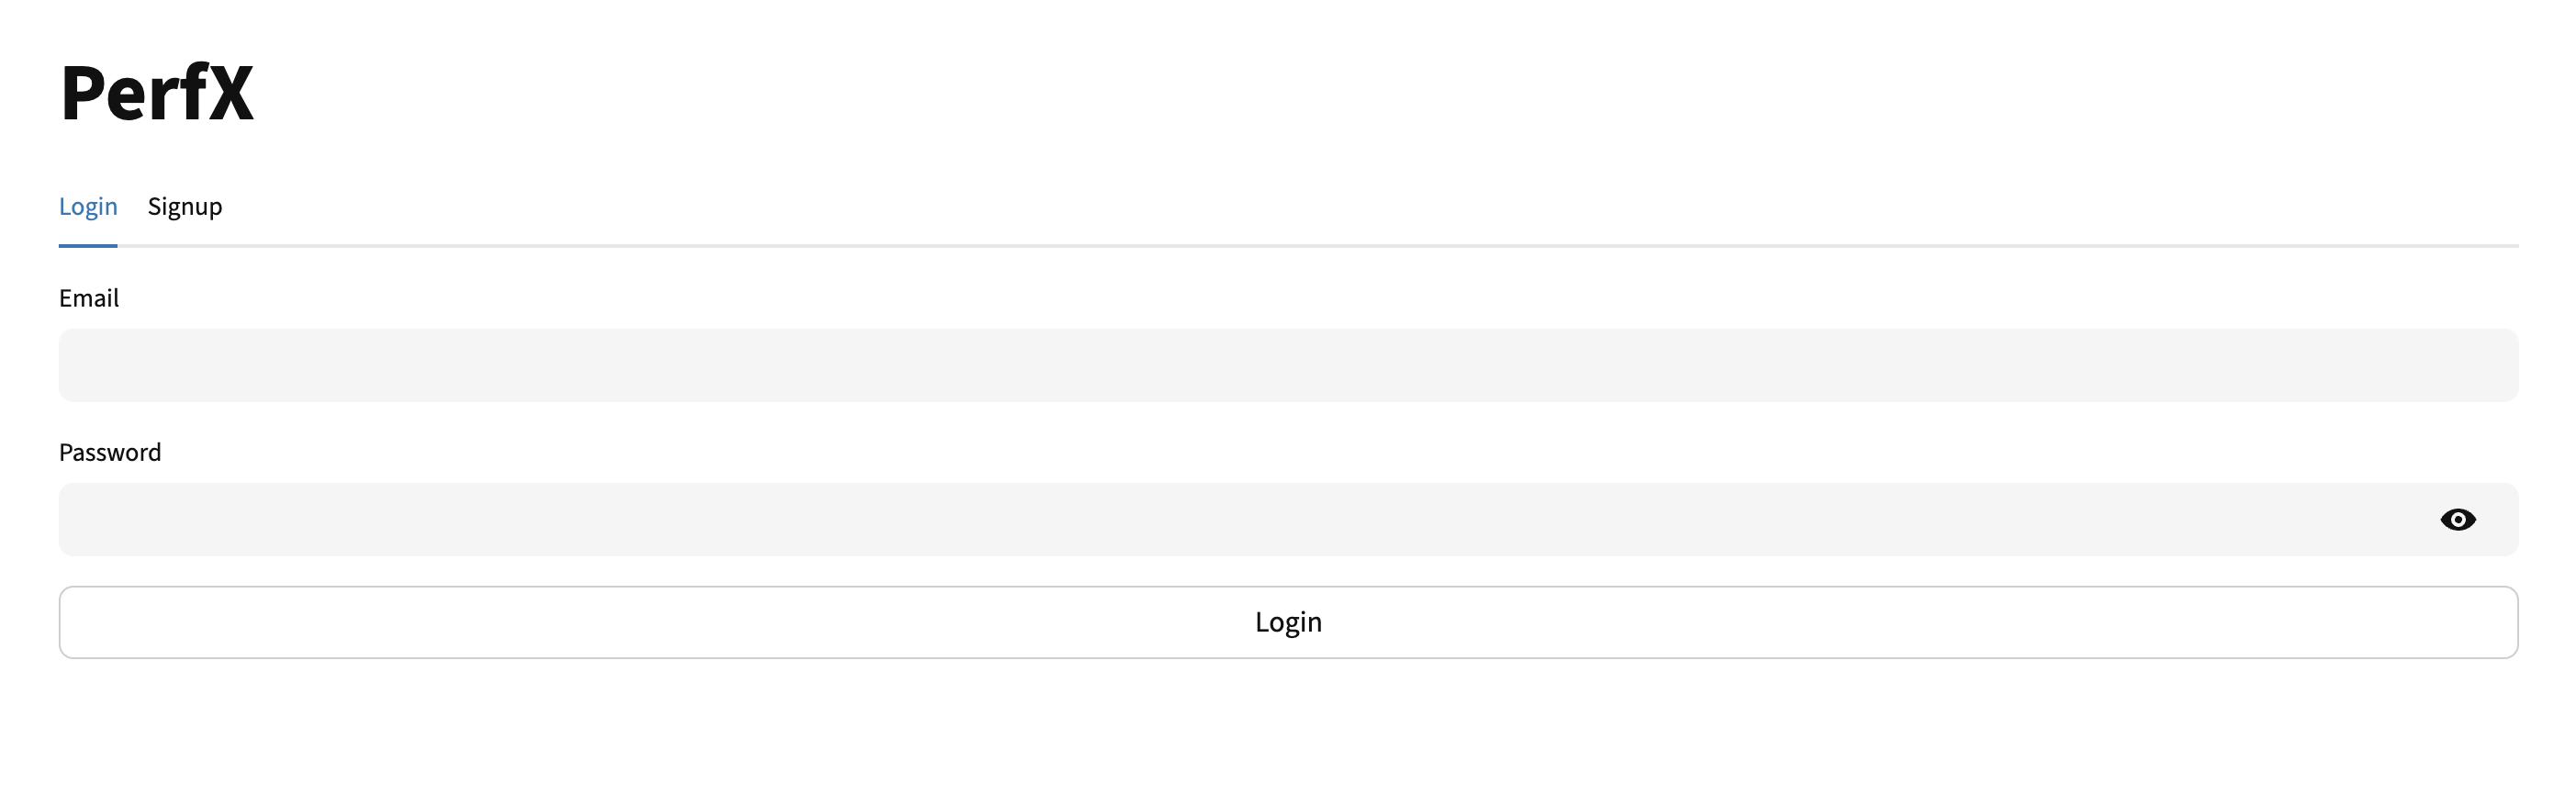
\includegraphics[width=0.8\textwidth]{figs/frontend_auth.png}
    \caption{Login page of the dashboard}
    \label{fig:auth_frontend}
\end{figure}

\subsection{Project Management}

Once logged in, a user sees their existing projects and can add or remove projects from the same page. When a new project is created, the dashboard displays the unique project ID that the developer needs to use when initializing the mobile SDK in their Android application.

\begin{figure}[H]
    \centering
    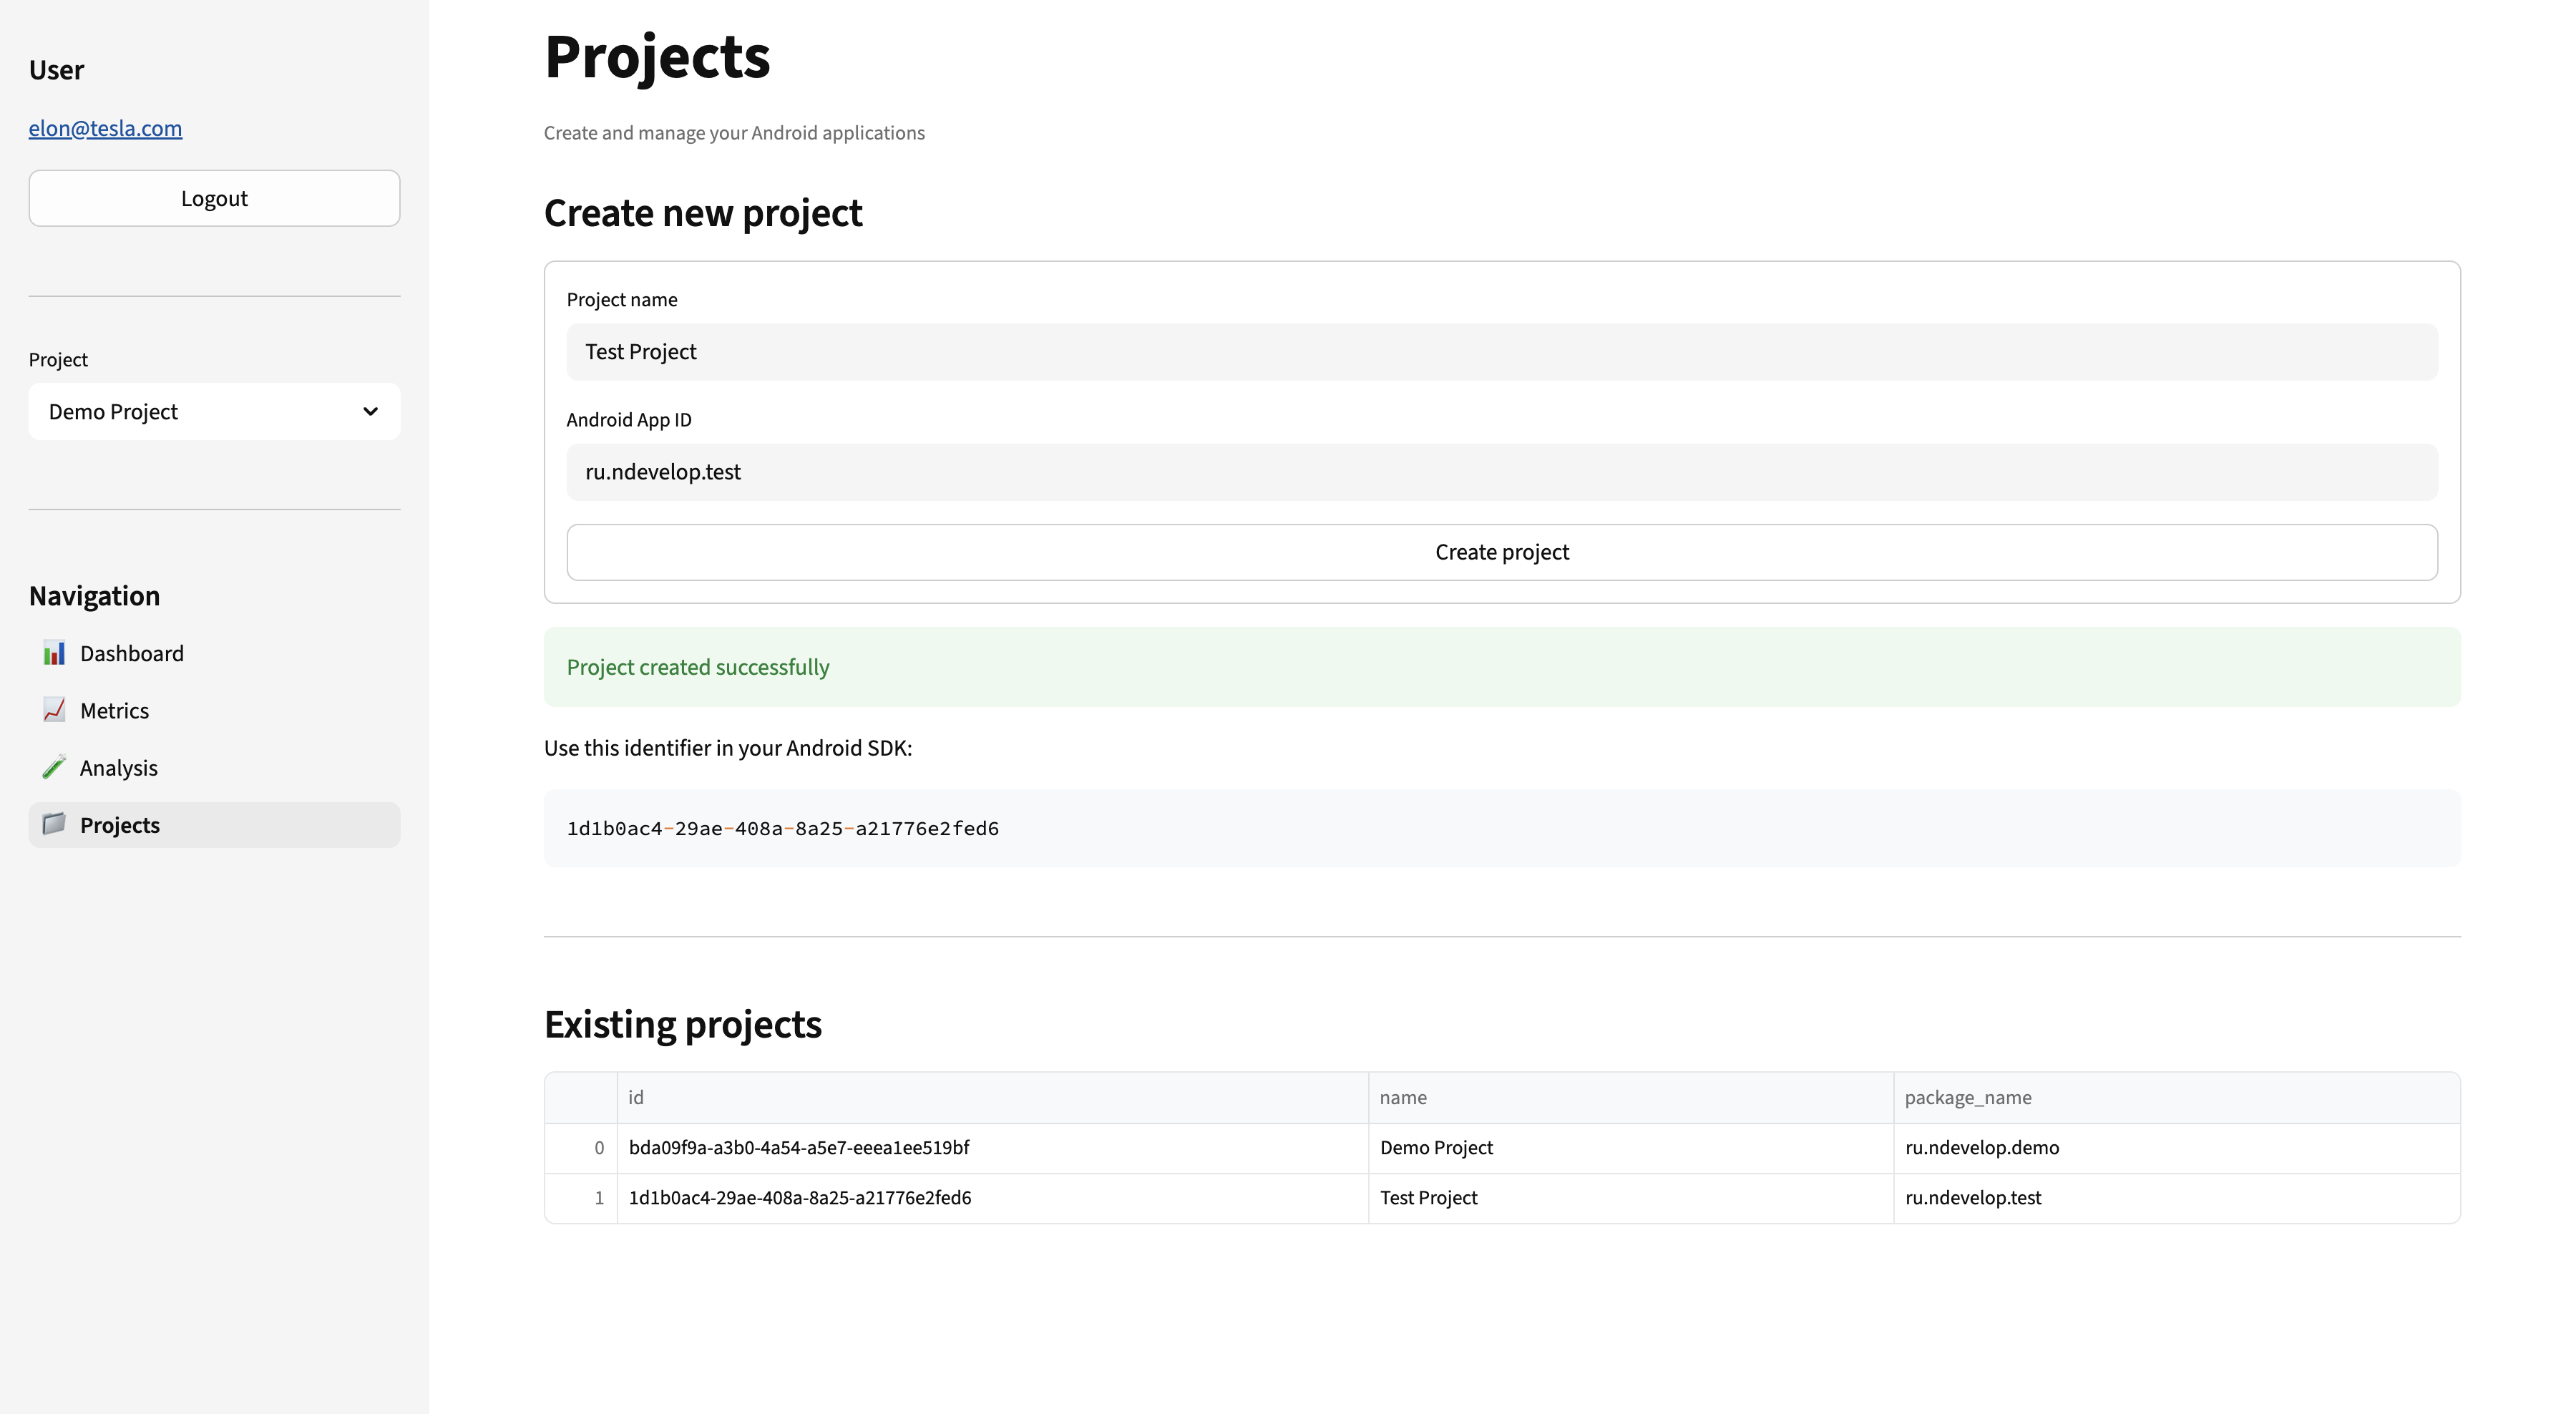
\includegraphics[width=0.8\textwidth]{figs/frontend_projects.png}
    \caption{Project list page}
    \label{fig:frontend_projects}
\end{figure}

\subsection{Metrics Explorer}

The metrics explorer presents the raw data in a table, where each measurement appears with its timestamp, value, and metadata. The table can be exported to CSV for deeper analysis in tools such as Excel or Jupyter Notebook. This helps with debugging and with one-off analyses.

\begin{figure}[H]
    \centering
    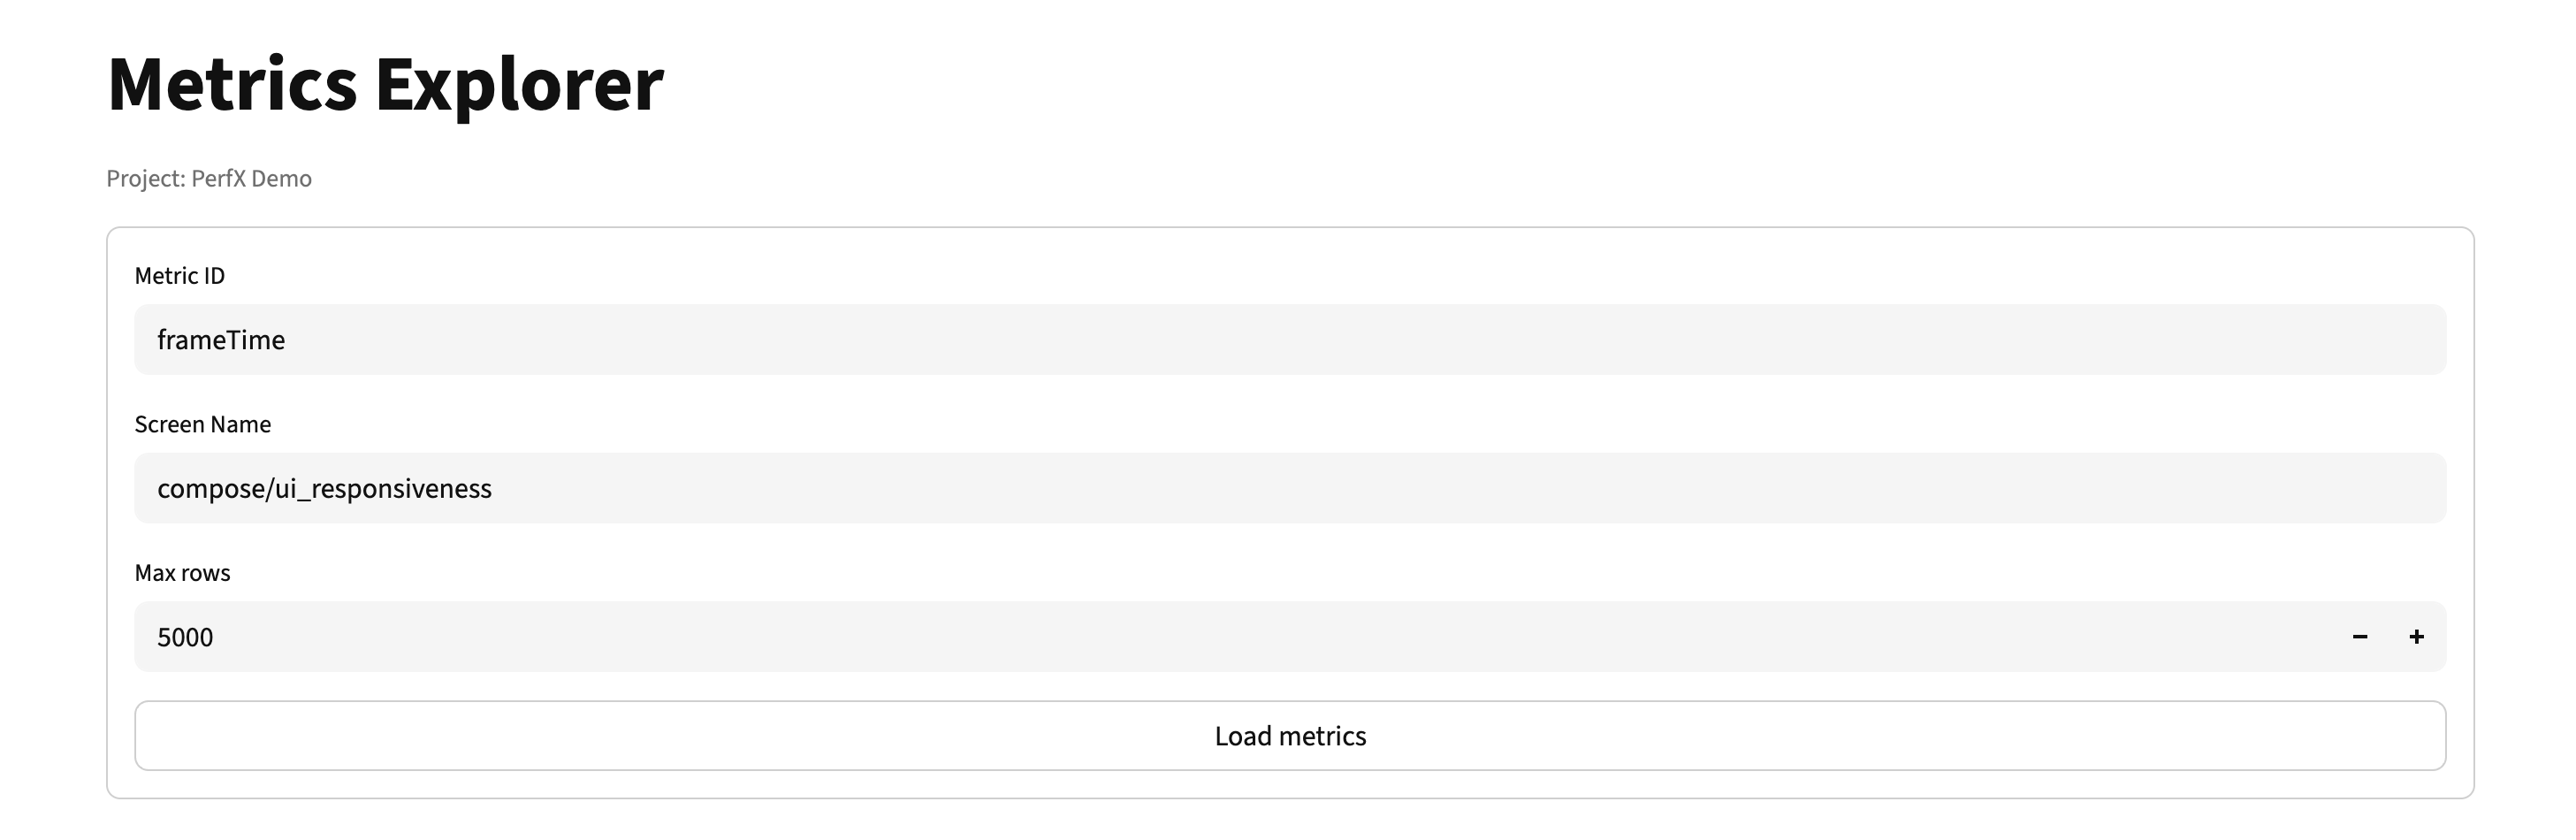
\includegraphics[width=0.8\textwidth]{figs/frontend_metrics_1.png}
    \caption{Metrics Explorer: filter selection}
    \label{fig:frontend_metrics_1}
\end{figure}

\begin{figure}[H]
    \centering
    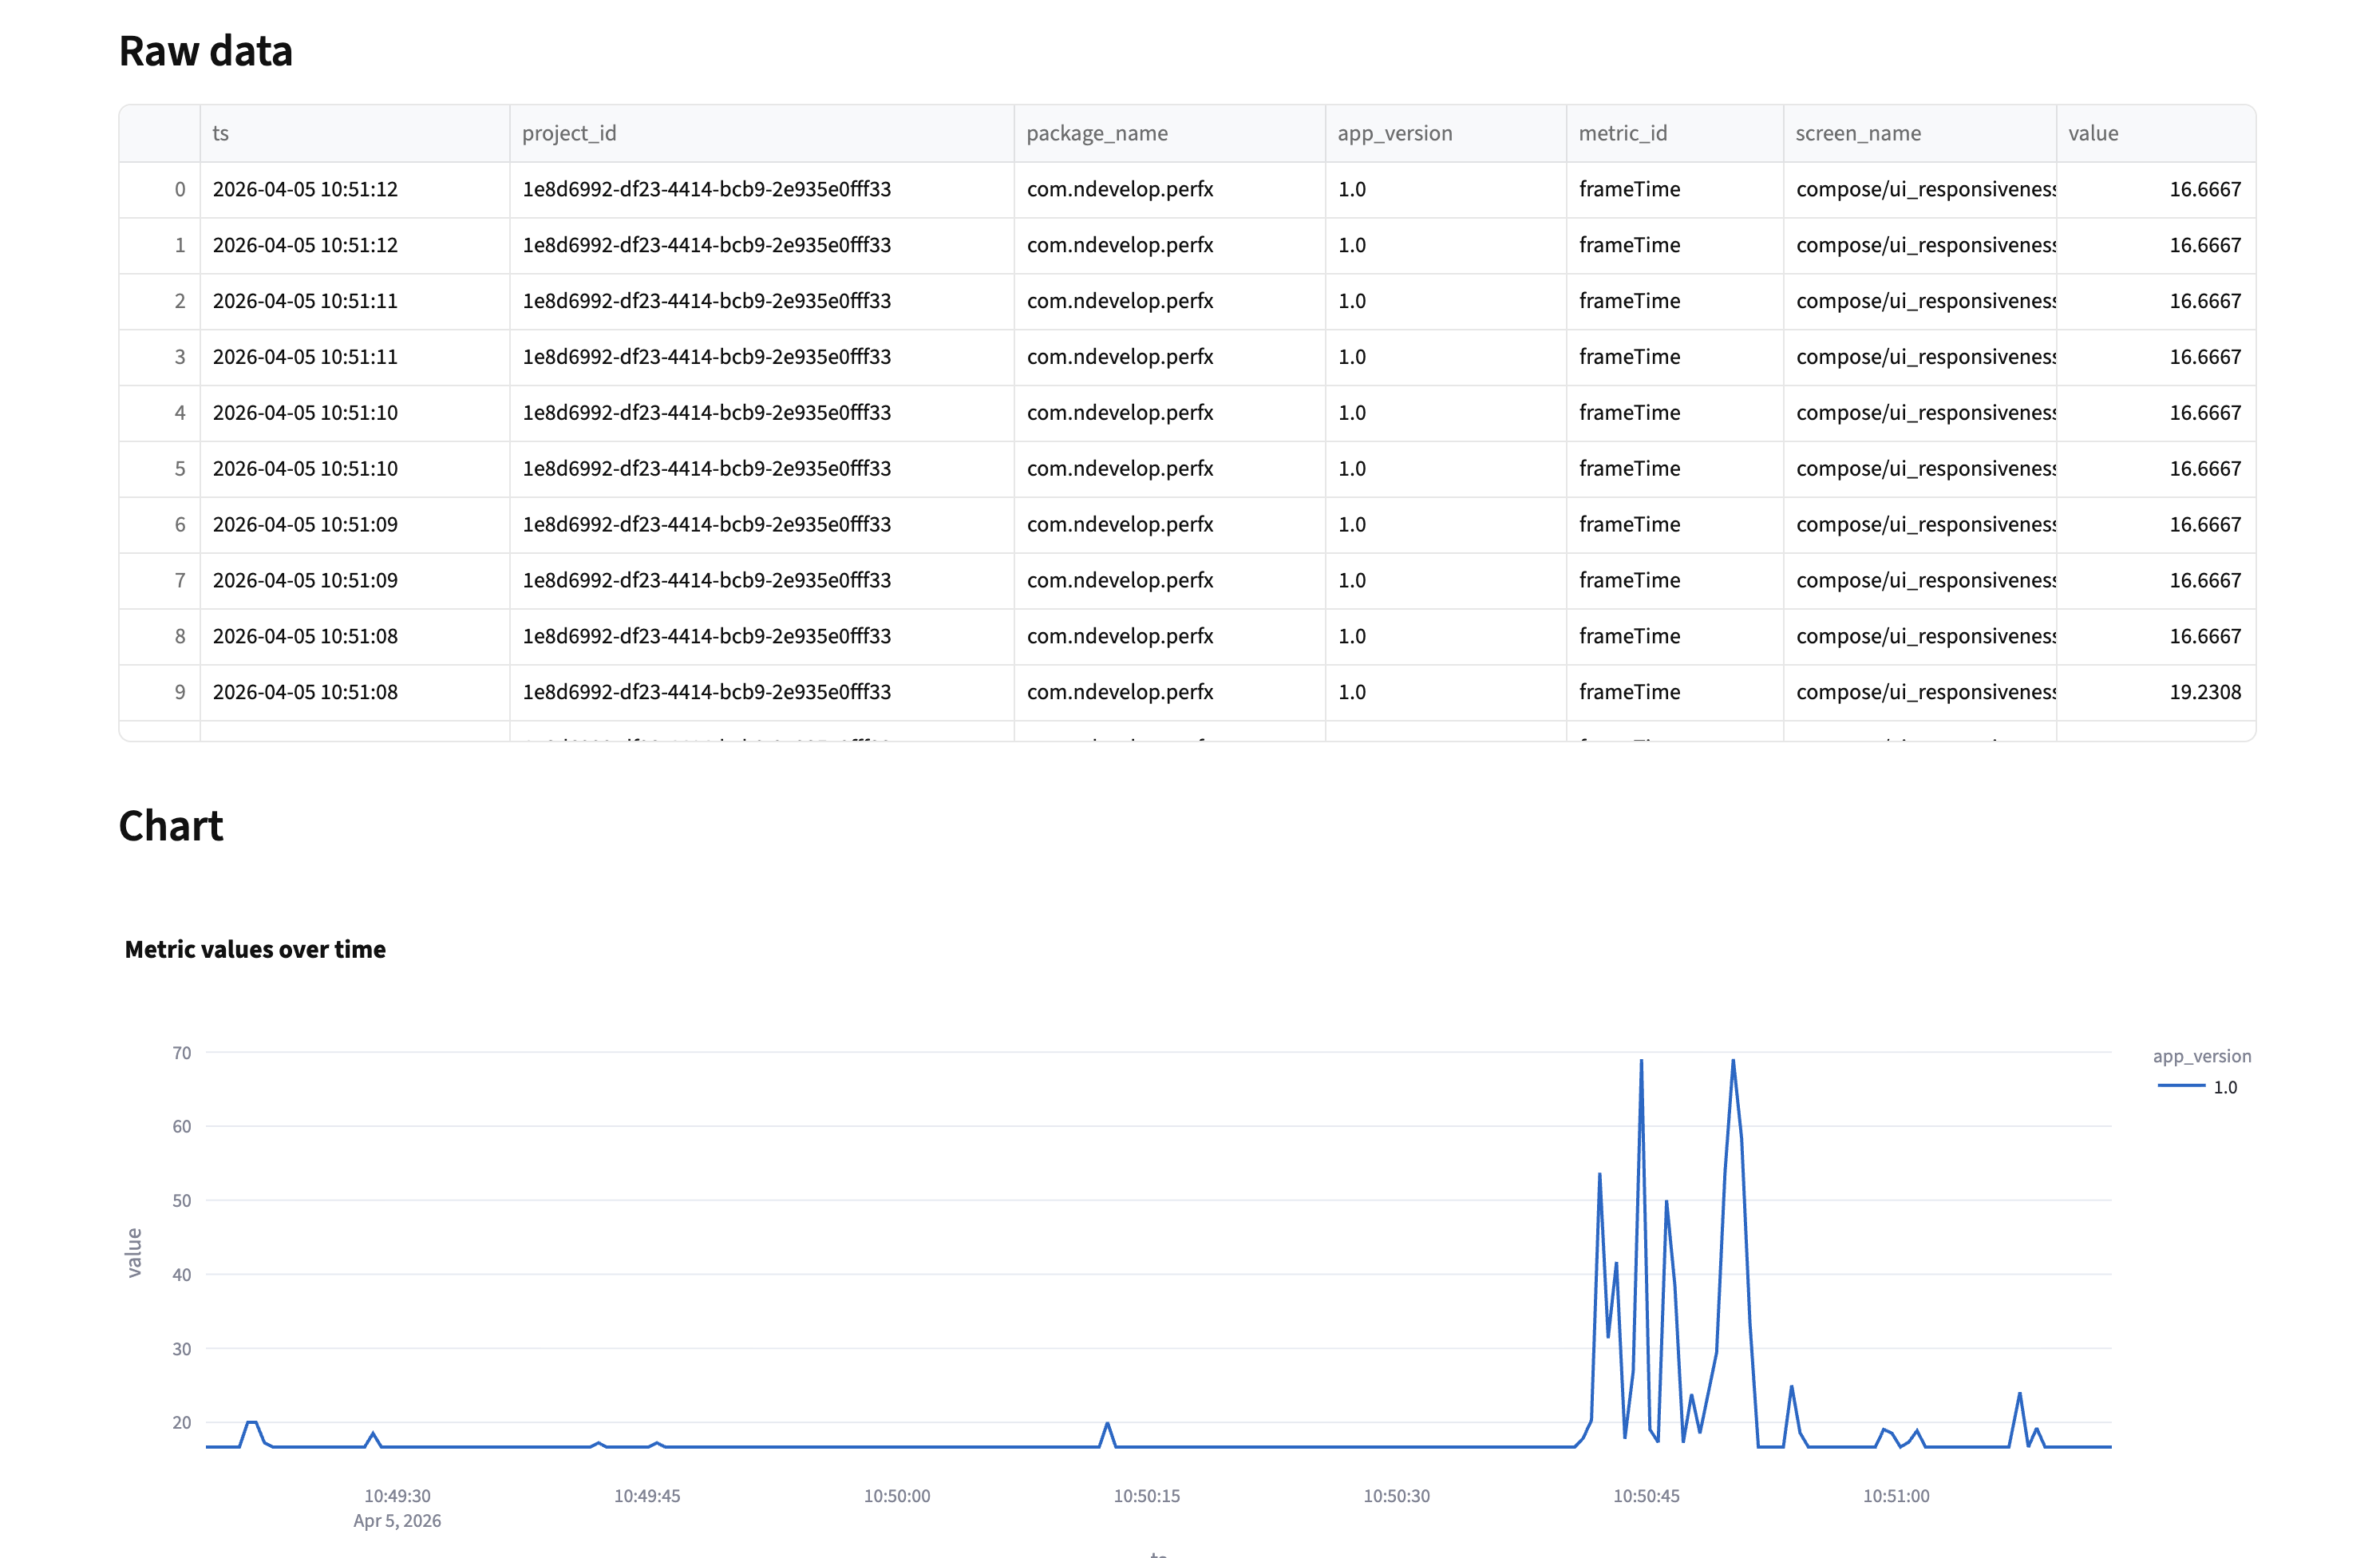
\includegraphics[width=0.8\textwidth]{figs/frontend_metrics_2.png}
    \caption{Metrics Explorer: frame time chart with a detected regression}
    \label{fig:frontend_metrics_2}
\end{figure}

\subsection{Regressions}

The regressions page lists every regression that the detection pipeline has reported for the selected project. Each row shows the affected metric, screen, and device cohort, the version pair that was compared, the degradation, and whether the regression is open or closed. A summary at the top of the page counts how many regressions are open and how many are closed. From the same page a developer can filter the list and close a regression once it has been handled.

\begin{figure}[H]
    \centering
    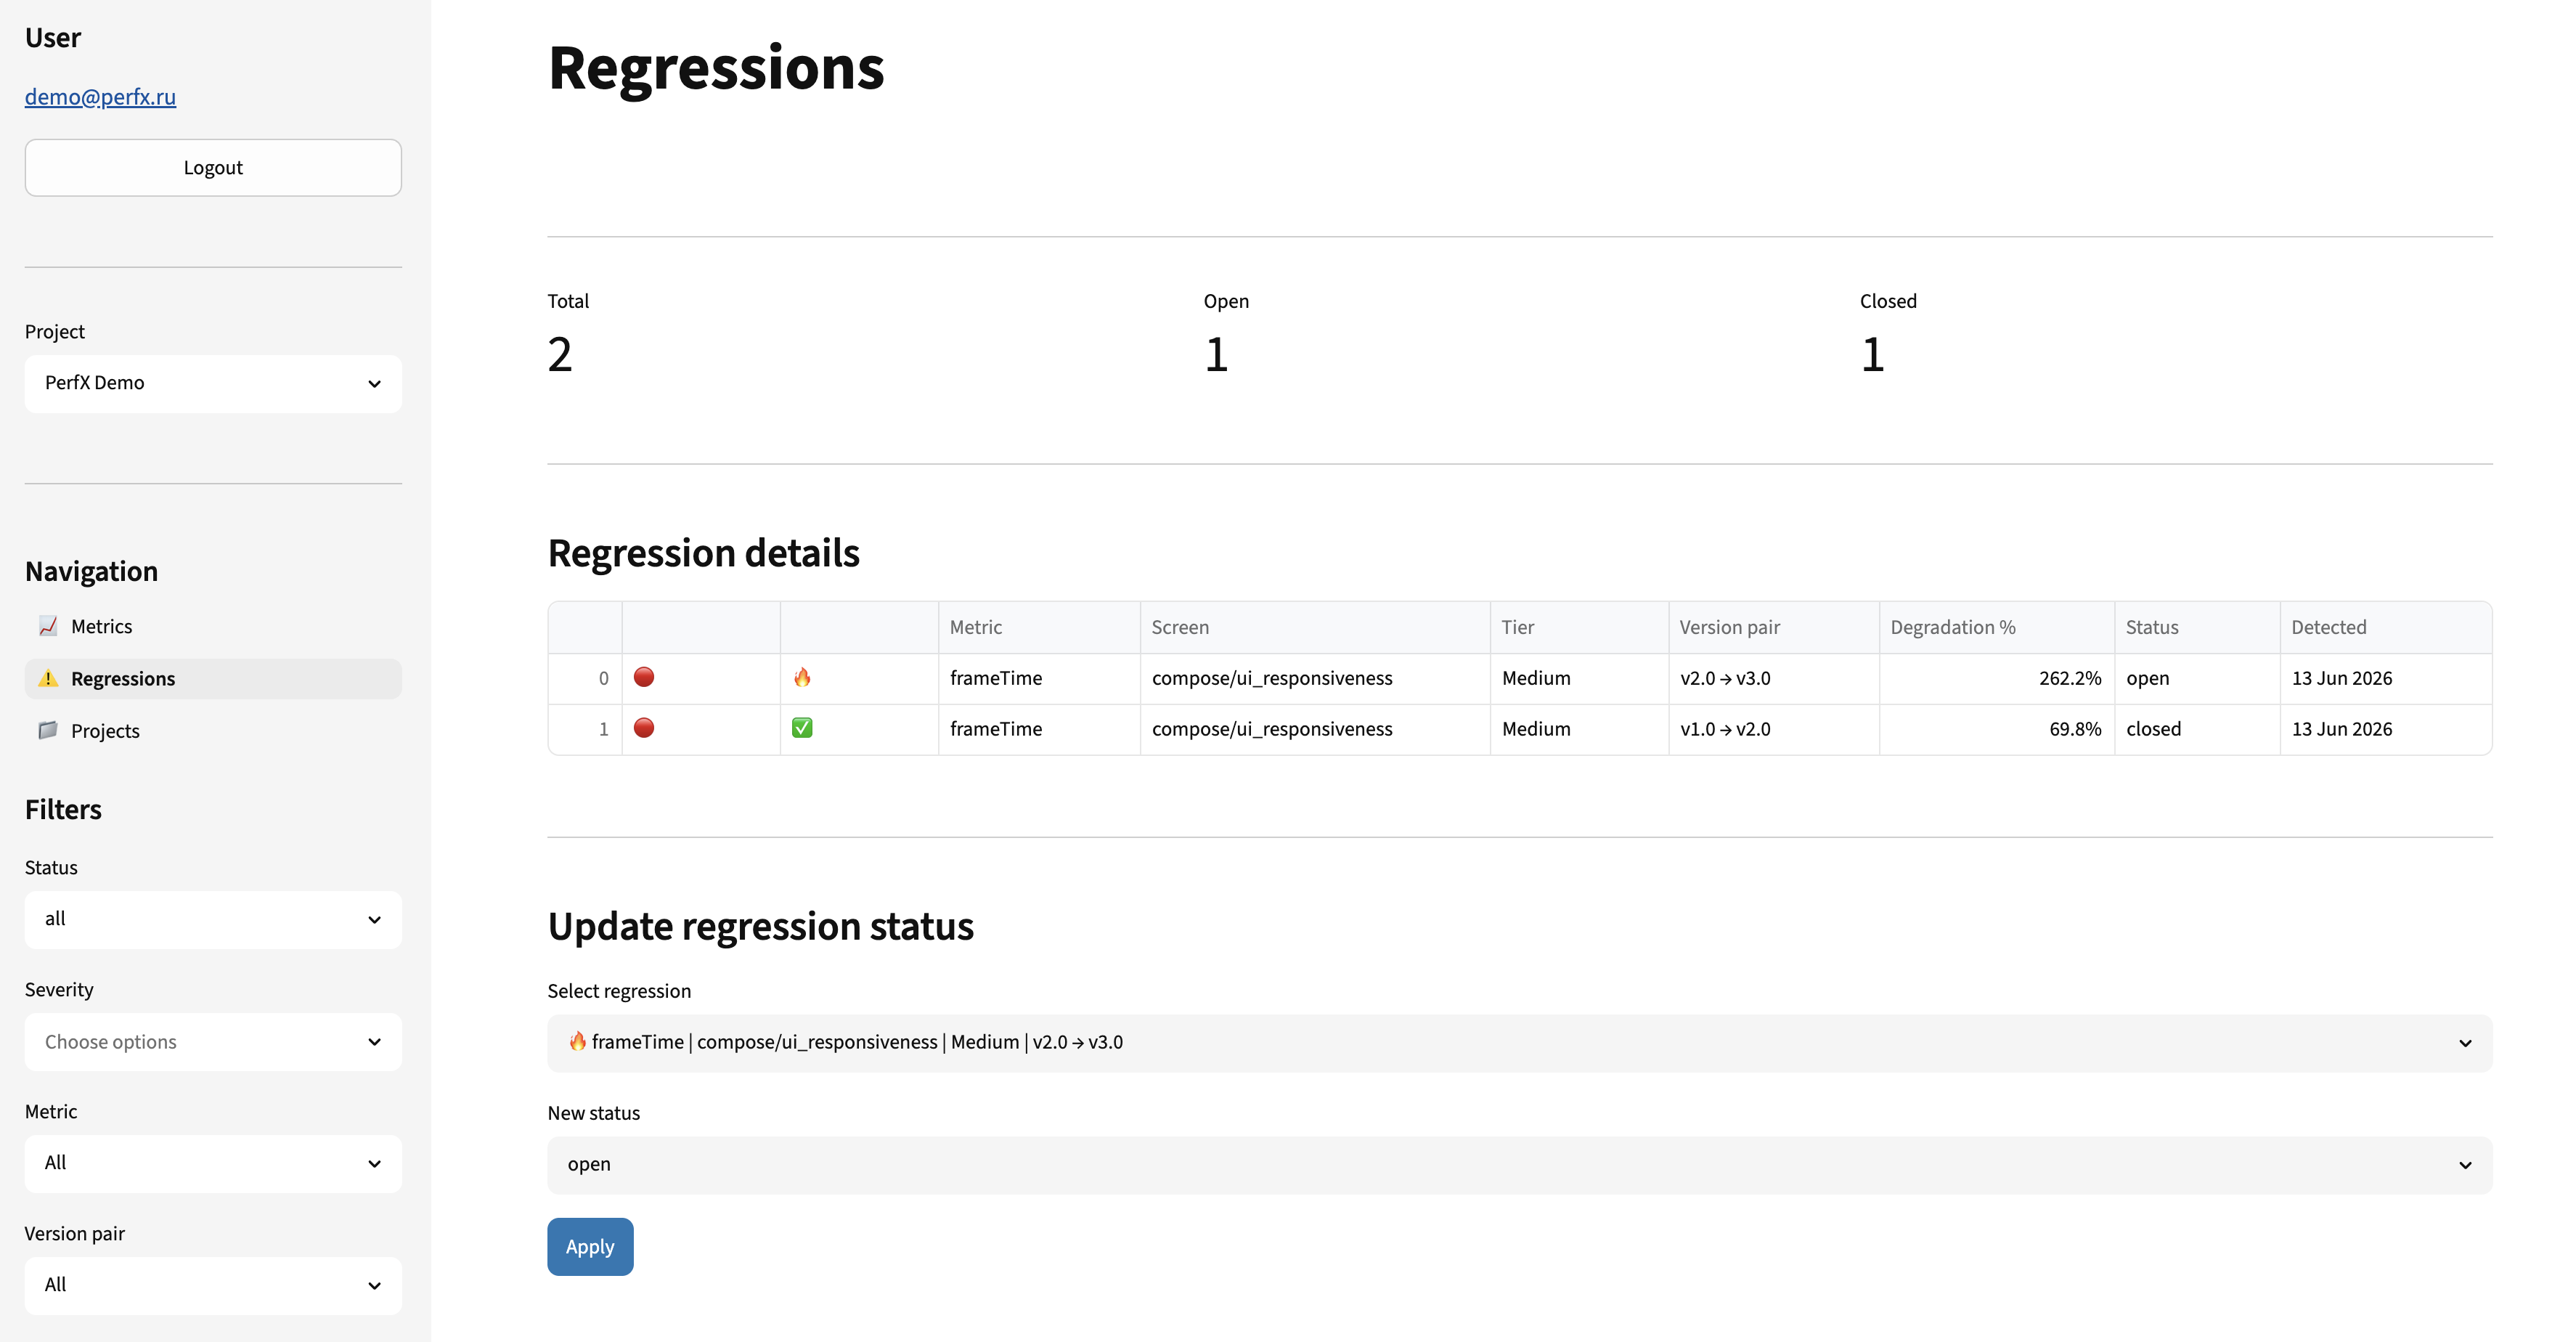
\includegraphics[width=\textwidth]{figs/regressions_page.png}
    \caption{Regressions page of the dashboard}
    \label{fig:regressions_page}
\end{figure}

Developers can also receive regression alerts in messenger. Each message reports the affected metric, screen, and device cohort, the compared version pair, and the magnitude of the degradation.

\begin{figure}[H]
    \centering
    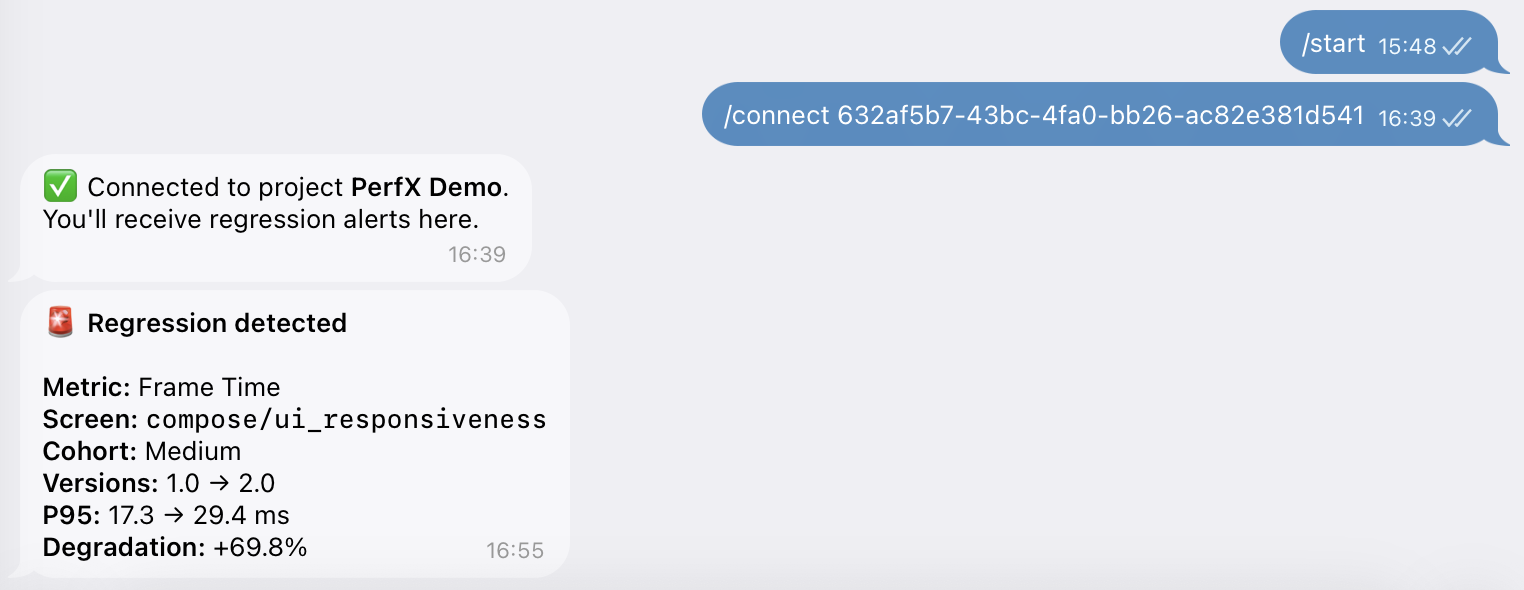
\includegraphics[width=0.75\textwidth]{figs/messaging_alert.png}
    \caption{Regression alert delivered to a messaging app}
    \label{fig:messaging_alert}
\end{figure}

% \newpage


\section{Summary}

This chapter described the implementation of all four system components. The mobile SDK was built as a Kotlin Android library that collects six performance metrics, buffers the data in a two-tier storage layer, and transmits it to the backend in batches. The Backend receives the data and stores it in two separate databases: ClickHouse for time-series metrics and PostgreSQL for user and project metadata. The regression detection pipeline was implemented as a Python service that computes per-version P95 values using ClickHouse aggregation queries and flags regressions when the relative P95 shift between consecutive releases exceeds the configured threshold. Finally, the frontend was built with Streamlit and lets developers explore the collected metrics and review detected regressions. The next chapter evaluates how well this system works in practice.
